\documentclass[9pt]{beamer}
\usetheme{metropolis}
\usepackage{amsmath}
\usepackage{amssymb}
\usepackage{graphicx}
\usepackage{booktabs}
\usepackage{xcolor}
\usepackage{tikz}
\usetikzlibrary{arrows,positioning,shapes.geometric,calc}

% Define color palette matching our project design system
\definecolor{primary}{HTML}{1abc9c}    % Deep Teal
\definecolor{secondary}{HTML}{3498db}  % Astro Blue
\definecolor{darkbg}{HTML}{2c3e50}     % Slate Blue
\definecolor{accent}{HTML}{e67e22}     % Orange

\setbeamercolor{palette primary}{bg=darkbg, fg=white}
\setbeamercolor{palette secondary}{bg=primary, fg=white}
\setbeamercolor{palette tertiary}{bg=secondary, fg=white}
\setbeamercolor{structure}{fg=primary}
\setbeamercolor{alerted text}{fg=accent}

\title{Physics-Informed Machine Learning (PIML)}
\subtitle{Bridging Empirical Data Science and Fundamental Physical Laws}
\author{Astronomy Club}
\date{\today}

\begin{document}

\maketitle

% Slide 2: Tutorial Roadmap
\begin{frame}{Tutorial Roadmap}
  This tutorial teaches the foundational concepts of Physics-Informed Machine Learning (PIML) and how to apply them to astrophysical systems:
  \begin{description}
    \item[Module 1:] \textbf{The PIML Paradigm Shift}
      \begin{itemize}
        \item Limitations of pure data-driven machine learning and the core philosophy of physics integration.
      \end{itemize}
    \item[Module 2:] \textbf{Enforcing Physics Constraints}
      \begin{itemize}
        \item Soft constraints (loss regularization), hard constraints (architectural design), and feature symmetries.
      \end{itemize}
    \item[Module 3:] \textbf{Automatic Differentiation (Autograd)}
      \begin{itemize}
        \item How neural networks compute exact physical derivatives to evaluate differential equations.
      \end{itemize}
    \item[Module 4:] \textbf{Case Study: Physics-Informed Rate Modeling}
      \begin{itemize}
        \item Restricting parameter spaces and building constrained neural models (Task 13).
      \end{itemize}
    \item[Module 5:] \textbf{Case Study: Convolved DTD Solvers}
      \begin{itemize}
        \item Integrating numerical convolved integrals into deep learning backpropagation (Task 15).
      \end{itemize}
  \end{description}
\end{frame}

% Module 1 Header
\begin{frame}[plain]
  \vfill
  \centering
  \begin{beamercolorbox}[sep=8pt,center,shadow=true,rounded=true]{palette primary}
    \usebeamerfont{title}\textbf{Module 1: The PIML Paradigm Shift}
  \end{beamercolorbox}
  \vfill
\end{frame}

% Slide 4: The Limitations of Pure Machine Learning
\begin{frame}{The Limitations of Pure Machine Learning}
  Standard machine learning models (like multi-layer perceptrons, decision trees, or random forests) are purely data-driven. They excel at finding correlations, but fail in physical sciences due to key limitations:
  \begin{description}
    \item[1. Physical Violations:] Data-driven models do not respect physical laws. A standard classifier might predict negative probabilities, violate conservation of energy, or output non-zero rates for mathematically impossible conditions.
    \item[2. Out-of-Distribution Failure:] Deep neural networks are excellent interpolators but poor extrapolators. If tested outside the boundaries of the training set, their predictions decay rapidly into unphysical regimes.
    \item[3. Massive Data Requirements:] Purely data-driven models require large training datasets to learn simple relationships (like $1/r^2$ gravity fields), which is problematic for rare astrophysical transients.
    \item[4. Lack of Physical Interpretability:] Black-box models only yield relative feature sensitivities, not physical parameters, units, or rate coefficients.
  \end{description}
\end{frame}

% Slide 5: What is Physics-Informed Machine Learning?
\begin{frame}{What is Physics-Informed Machine Learning?}
  \textbf{Physics-Informed Machine Learning (PIML)} blends empirical observations (data) with prior scientific knowledge (theoretical models, symmetries, boundary conditions, or differential equations).
  \begin{center}
    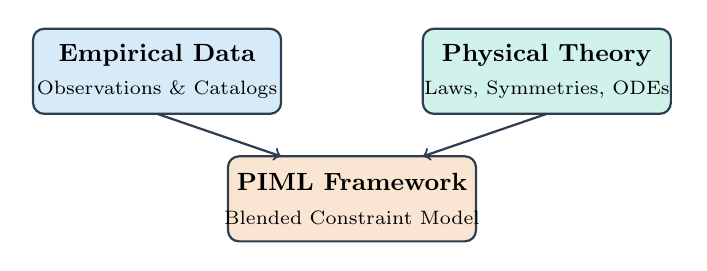
\begin{tikzpicture}[scale=0.9]
      \draw[draw=darkbg, fill=secondary!20, thick, rounded corners] (0,0) rectangle (3.5, 1.2);
      \node[align=center] at (1.75, 0.6) {\small \textbf{Empirical Data} \\ \scriptsize Observations \& Catalogs};
      
      \draw[draw=darkbg, fill=primary!20, thick, rounded corners] (5.5,0) rectangle (9, 1.2);
      \node[align=center] at (7.25, 0.6) {\small \textbf{Physical Theory} \\ \scriptsize Laws, Symmetries, ODEs};
      
      \draw[draw=darkbg, fill=accent!20, thick, rounded corners] (2.75,-1.8) rectangle (6.25, -0.6);
      \node[align=center] at (4.5, -1.2) {\small \textbf{PIML Framework} \\ \scriptsize Blended Constraint Model};
      
      \draw[thick, ->, draw=darkbg] (1.75, 0) -- (3.5, -0.6);
      \draw[thick, ->, draw=darkbg] (7.25, 0) -- (5.5, -0.6);
    \end{tikzpicture}
  \end{center}
  By constraining the search space of the model to only include physically valid functions, PIML:
  \begin{itemize}
    \item Restricts models to physically realistic boundaries.
    \item Reduces the volume of training data required by orders of magnitude.
    \item Generalizes and extrapolates reliably outside training regions.
  \end{itemize}
\end{frame}

% Slide 6: Pure Physics vs. Pure ML vs. PIML
\begin{frame}{Comparison Matrix}
  \begin{table}
    \centering
    \begin{tabular}{r c c c}
      \toprule
      \textbf{Metric} & \textbf{Pure Physics} & \textbf{Pure ML} & \textbf{PIML} \\
      \midrule
      \textbf{Data Needs} & None (analytical) & Extremely High & Low to Moderate \\
      \textbf{Physics Respect} & Perfect ($100\%$) & None (fails limits) & Guaranteed (by design) \\
      \textbf{Generalizability} & Perfect (general laws) & Poor (interpolation only) & High (extrapolates) \\
      \textbf{Inference Speed} & Slow (numeric integrals) & Extremely Fast & Extremely Fast \\
      \textbf{Noisy Data Robustness} & Low & High & High \\
      \bottomrule
    \end{tabular}
    \caption{Comparative analysis of modeling paradigms in astronomy.}
  \end{table}
\end{frame}

% Module 2 Header
\begin{frame}[plain]
  \vfill
  \centering
  \begin{beamercolorbox}[sep=8pt,center,shadow=true,rounded=true]{palette primary}
    \usebeamerfont{title}\textbf{Module 2: Enforcing Physics Constraints}
  \end{beamercolorbox}
  \vfill
\end{frame}

% Slide 8: Categories of Physics Integration
\begin{frame}{Categories of Physics Integration}
  We can inject physical theory into machine learning models at three distinct levels:
  \begin{description}
    \item[1. Feature-Level (Input Integration):]
      Transform input features to satisfy symmetries and physical invariances.
      \begin{itemize}
        \item \textbf{Example:} Enforce rotational invariance by converting Cartesian coordinates $(x, y, z)$ to spherical coordinates $(r, \theta, \phi)$ before training.
      \end{itemize}
    \item[2. Loss-Level (Soft Constraints):]
      Add physical residuals (differential equations or boundaries) to the loss function. The network is penalized for violating physical laws.
    \item[3. Architecture-Level (Hard Constraints):]
      Design layers or equations inside the network that guarantee physical laws are satisfied exactly, regardless of training epochs.
  \end{description}
\end{frame}

% Slide 9: Loss-Level Constraints (Soft Constraints)
\begin{frame}{Loss-Level Constraints (Soft Constraints)}
  Consider a system governed by a differential equation:
  $$f(\mathbf{x}, u(\mathbf{x})) = 0$$
  where $u(\mathbf{x})$ is the physical quantity we wish to model, and $\mathbf{x}$ are inputs.
  \begin{block}{Composite Loss Function}
    To enforce this law, we define a composite loss:
    $$\mathcal{L} = \mathcal{L}_{\text{data}} + \lambda \cdot \mathcal{L}_{\text{physics}}$$
    \begin{align*}
      \mathcal{L}_{\text{data}} &= \frac{1}{N_d} \sum_{i=1}^{N_d} \|u(\mathbf{x}_i) - u_{\text{observed}, i}\|^2 \\
      \mathcal{L}_{\text{physics}} &= \frac{1}{N_{\text{col}}} \sum_{j=1}^{N_{\text{col}}} \|f(\mathbf{x}_j, u(\mathbf{x}_j))\|^2
    \end{align*}
  \end{block}
  The regularization coefficient $\lambda > 0$ balances data matching and physics compliance. This constraint is \textbf{soft} because the optimizer might accept small physical violations to better fit noisy training data.
\end{frame}

% Slide 10: Architecture-Level Constraints (Hard Constraints)
\begin{frame}{Architecture-Level Constraints (Hard Constraints)}
  Soft constraints can still violate physical boundaries if the loss optimization converges to a local minimum. To ensure physical laws are met exactly, we build them directly into the network architecture:
  \begin{block}{Examples of Architectural Integration}
    \begin{itemize}
      \item \textbf{Non-Negativity Constraints:} If a physical quantity (like mass or rate) must be strictly non-negative, we pass the network's raw outputs through an exponential function:
        $$u_{\text{physical}} = e^{u_{\text{raw}}} \quad \implies \quad u_{\text{physical}} > 0 \text{ always}$$
      \item \textbf{Probability Conservation:} Enforces that predicted class assignments sum to $1.0$ by applying a Softmax layer at the final output:
        $$\sum_c P_c = 1.0 \text{ always}$$
      \item \textbf{Energy Conservation:} Hard-code an energy conservation block $E_{\text{kinetic}} + E_{\text{potential}} = E_{\text{total}}$ as an analytical layer.
    \end{itemize}
  \end{block}
\end{frame}

% Module 3 Header
\begin{frame}[plain]
  \vfill
  \centering
  \begin{beamercolorbox}[sep=8pt,center,shadow=true,rounded=true]{palette primary}
    \usebeamerfont{title}\textbf{Module 3: Automatic Differentiation (Autograd)}
  \end{beamercolorbox}
  \vfill
\end{frame}

% Slide 12: Automatic Differentiation (Autograd) in PIML
\begin{frame}{Automatic Differentiation (Autograd) in PIML}
  To evaluate differential equations (like $\frac{du}{dx}$) in a loss-level constraint, we must calculate the derivatives of our neural network's predictions with respect to its inputs.
  \begin{itemize}
    \item \textbf{Why not numerical differentiation?}
      Finite difference approximations ($\frac{u(x+\Delta x) - u(x)}{\Delta x}$) are computationally expensive (scale poorly with input dimension) and suffer from numerical truncation errors.
    \item \textbf{Why not analytical differentiation?}
      Calculating derivatives by hand for deep, non-linear networks is highly complex and impractical.
    \item \textbf{The PIML Solution: Autograd}
      Automatic differentiation tracks operations on a computational graph. It computes exact, analytical derivatives down to machine precision using the chain rule, scaling efficiently to high dimensions.
  \end{itemize}
\end{frame}

% Slide 13: Autograd Computational Flow
\begin{frame}{Autograd Computational Flow}
  Below is a schematic showing how automatic differentiation propagates gradients through a physical loss loop. Autograd calculates the exact physical derivative $\frac{du}{dx}$ and uses it to update the model weights $W$:
  \vfill
  \centering
  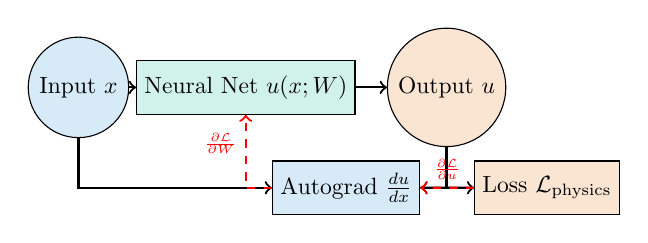
\begin{tikzpicture}[scale=0.85, every node/.style={transform shape}]
    % Graph nodes
    \node[circle, draw, fill=secondary!20] (input) at (0,0) {Input $x$};
    \node[draw, fill=primary!20, minimum height=0.8cm, minimum width=1.5cm] (nn) at (2.5,0) {Neural Net $u(x; W)$};
    \node[circle, draw, fill=accent!20] (output) at (5.5,0) {Output $u$};
    
    \node[draw, fill=secondary!20, minimum height=0.8cm, minimum width=1.5cm] (deriv) at (4,-1.5) {Autograd $\frac{du}{dx}$};
    \node[draw, fill=accent!20, minimum height=0.8cm] (loss) at (7,-1.5) {Loss $\mathcal{L}_{\text{physics}}$};
    
    % Forward paths
    \draw[->, thick] (input) -- (nn);
    \draw[->, thick] (nn) -- (output);
    \draw[->, thick] (output) |- (deriv);
    \draw[->, thick] (input) |- (deriv);
    \draw[->, thick] (deriv) -- (loss);
    
    % Backward gradient path
    \draw[->, dashed, red, thick] (loss) -- node[above] {\scriptsize $\frac{\partial \mathcal{L}}{\partial u}$} (deriv);
    \draw[->, dashed, red, thick] (deriv) -| node[left, pos=0.8] {\scriptsize $\frac{\partial \mathcal{L}}{\partial W}$} (nn);
  \end{tikzpicture}
  \vfill
\end{frame}

% Module 4 Header
\begin{frame}[plain]
  \vfill
  \centering
  \begin{beamercolorbox}[sep=8pt,center,shadow=true,rounded=true]{palette primary}
    \usebeamerfont{title}\textbf{Module 4: Case Study: Physics-Informed Rate Modeling}
  \end{beamercolorbox}
  \vfill
\end{frame}

% Slide 15: Constrained Parameter Estimation (Task 13)
\begin{frame}{Constrained Parameter Estimation (Task 13)}
  Let's examine the rate equation for Type Ia Supernovae:
  $$R_{\text{Ia}}(M_\star, \text{SFR}) = A \cdot M_{\star, 10} + B \cdot \text{SFR}$$
  where $A$ (delayed component) and $B$ (prompt component) are physical rates.
  \begin{block}{Enforcing Non-Negativity}
    Because supernova rates cannot be negative, we must enforce $A \ge 0$ and $B \ge 0$ during training.
    We build a Physics-Informed Neural Network (PINN) rate model. Rather than fitting $A$ and $B$ directly, we define two unbounded neural network parameters $\tilde{A}, \tilde{B} \in \mathbb{R}$. We then map them using an exponential layer:
    $$A = e^{\tilde{A}}, \quad B = e^{\tilde{B}}$$
    This guarantees that $A$ and $B$ remain strictly positive throughout the gradient descent optimization, preventing unphysical negative rates.
  \end{block}
\end{frame}

% Slide 16: PINN Rate Model Architecture
\begin{frame}{PINN Rate Model Architecture}
  Below is the network architecture for our Task 13 PINN. Unbounded parameters ($\tilde{A}, \tilde{B}$) are transformed via exponential layers to satisfy the physical positivity bounds of the rate equation:
  \vfill
  \centering
  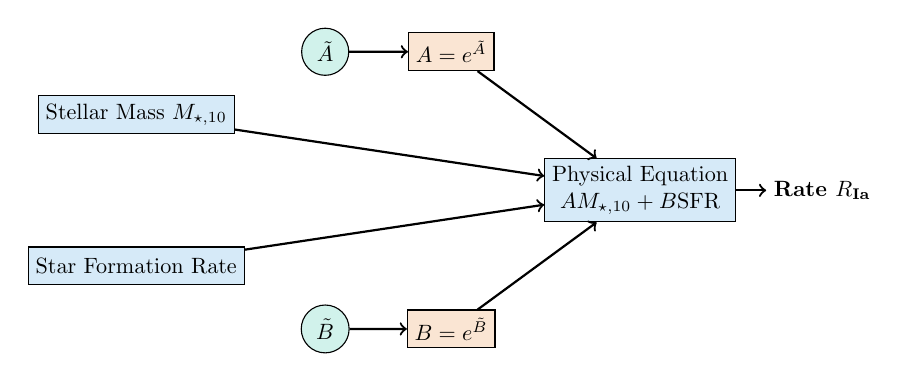
\begin{tikzpicture}[scale=0.8, every node/.style={transform shape}]
    % Inputs
    \node[draw, fill=secondary!20, minimum height=0.6cm] (mass) at (0, 1.2) {Stellar Mass $M_{\star, 10}$};
    \node[draw, fill=secondary!20, minimum height=0.6cm] (sfr) at (0, -1.2) {Star Formation Rate};
    
    % Weights
    \node[circle, draw, fill=primary!20] (a_raw) at (3, 2.2) {$\tilde{A}$};
    \node[circle, draw, fill=primary!20] (b_raw) at (3, -2.2) {$\tilde{B}$};
    
    % Exponential mapping (constraints)
    \node[draw, fill=accent!20, minimum height=0.6cm] (a_exp) at (5, 2.2) {$A = e^{\tilde{A}}$};
    \node[draw, fill=accent!20, minimum height=0.6cm] (b_exp) at (5, -2.2) {$B = e^{\tilde{B}}$};
    
    % Rate Equation node
    \node[draw, fill=secondary!20, minimum height=1cm, text width=2.8cm, align=center] (rate) at (8, 0) {Physical Equation \\ $A M_{\star, 10} + B \text{SFR}$};
    \node[right] (output) at (10, 0) {\textbf{Rate $R_{\text{Ia}}$}};
    
    % Connections
    \draw[->, thick] (a_raw) -- (a_exp);
    \draw[->, thick] (b_raw) -- (b_exp);
    \draw[->, thick] (mass) -- (rate);
    \draw[->, thick] (sfr) -- (rate);
    \draw[->, thick] (a_exp) -- (rate);
    \draw[->, thick] (b_exp) -- (rate);
    \draw[->, thick] (rate) -- (output);
  \end{tikzpicture}
  \vfill
\end{frame}

% Module 5 Header
\begin{frame}[plain]
  \vfill
  \centering
  \begin{beamercolorbox}[sep=8pt,center,shadow=true,rounded=true]{palette primary}
    \usebeamerfont{title}\textbf{Module 5: Case Study: Convolved DTD Solvers}
  \end{beamercolorbox}
  \vfill
\end{frame}

% Slide 18: Numerical Convolved Integral Solvers (Task 15)
\begin{frame}{Numerical Convolved Integral Solvers (Task 15)}
  In Task 15, we model the rate of Type Ia Supernovae in a galaxy as the convolved product of its Star Formation History ($\text{SFR}(t)$) and the Delay Time Distribution ($\Psi$):
  $$R_{\text{Ia}}(t) = \int_0^t \text{SFR}(t - \tau) \Psi(\tau) d\tau = \int_0^t \text{SFR}(t - \tau) \tau^{-\gamma} d\tau$$
  \begin{itemize}
    \item \textbf{The Challenge:} Standard neural networks cannot evaluate continuous integrals natively.
    \item \textbf{The PIML Solution:} We discretize the convolution integral on a fine cosmic time grid ($t_k = k \cdot \Delta t$) and formulate it as a vectorized matrix multiplication:
      $$\mathbf{r} = \mathbf{S} \boldsymbol{\psi}(\gamma) \cdot \Delta t$$
      where $\mathbf{S}$ is a matrix of lookback SFR values for each galaxy, and $\boldsymbol{\psi}(\gamma)$ is the DTD vector.
    \item We parameterize the power-law slope $\gamma$ as a PyTorch weight. Backpropagation flows from the likelihood loss directly through the convolved rate vector back to the physical parameter $\gamma$.
  \end{itemize}
\end{frame}

% Slide 19: Convolved DTD Solver Flowchart
\begin{frame}{Convolved DTD Solver Flowchart}
  Below is the computational pipeline of our convolved solver. Gradients flow from the loss function through the numerical convolution block back to the physical parameter $\gamma$:
  \vfill
  \centering
  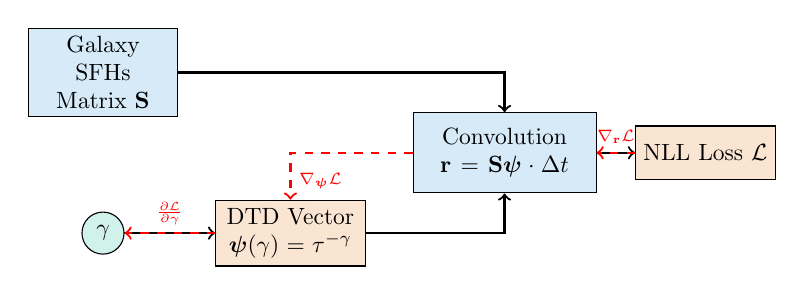
\begin{tikzpicture}[scale=0.85, every node/.style={transform shape}]
    % Inputs
    \node[draw, fill=secondary!20, minimum height=0.8cm, text width=2cm, align=center] (sfh) at (0, 1.2) {Galaxy SFHs \\ Matrix $\mathbf{S}$};
    \node[circle, draw, fill=primary!20] (gamma) at (0, -1.2) {$\gamma$};
    
    % DTD block
    \node[draw, fill=accent!20, minimum height=0.8cm, text width=2cm, align=center] (dtd) at (2.8, -1.2) {DTD Vector \\ $\boldsymbol{\psi}(\gamma) = \tau^{-\gamma}$};
    
    % Convolution Block
    \node[draw, fill=secondary!20, minimum height=1.2cm, text width=2.5cm, align=center] (conv) at (6, 0) {Convolution \\ $\mathbf{r} = \mathbf{S} \boldsymbol{\psi} \cdot \Delta t$};
    
    % Loss
    \node[draw, fill=accent!20, minimum height=0.8cm] (loss) at (9, 0) {NLL Loss $\mathcal{L}$};
    
    % Connections
    \draw[->, thick] (sfh) -| (conv);
    \draw[->, thick] (gamma) -- (dtd);
    \draw[->, thick] (dtd) -| (conv);
    \draw[->, thick] (conv) -- (loss);
    
    % Backpropagation arrows
    \draw[->, dashed, red, thick] (loss) -- node[above] {\scriptsize $\nabla_{\mathbf{r}}\mathcal{L}$} (conv);
    \draw[->, dashed, red, thick] (conv) -| node[right, pos=0.8] {\scriptsize $\nabla_{\boldsymbol{\psi}}\mathcal{L}$} (dtd);
    \draw[->, dashed, red, thick] (dtd) -- node[above] {\scriptsize $\frac{\partial\mathcal{L}}{\partial\gamma}$} (gamma);
  \end{tikzpicture}
  \vfill
\end{frame}

% Module 6 Header
\begin{frame}[plain]
  \vfill
  \centering
  \begin{beamercolorbox}[sep=8pt,center,shadow=true,rounded=true]{palette primary}
    \usebeamerfont{title}\textbf{Module 6: Summary \& Best Practices}
  \end{beamercolorbox}
  \vfill
\end{frame}

% Slide 21: Advanced Astrophysical Applications of PIML
\begin{frame}{Advanced Astrophysical Applications of PIML}
  Beyond rate modeling, Physics-Informed Machine Learning is revolutionizing contemporary research across multiple domains in astronomy:
  \begin{description}
    \item[1. Celestial Mechanics \& Exoplanets:]
      Training neural networks to predict exoplanetary orbits while enforcing Kepler's Laws or Hamiltonian energy conservation as hard constraints.
    \item[2. Stellar Atmospheres:]
      Accelerating complex radiative transfer codes. The neural network learns to map stellar parameters to output spectra while enforcing flux conservation.
    \item[3. Cosmology:]
      Predicting the growth of large-scale structure in the universe. The network replaces expensive N-body simulations while constrained by fluid dynamics equations (Euler and continuity equations).
  \end{description}
\end{frame}

% Slide 22: PIML Summary & Checklist
\begin{frame}{PIML Summary \& Checklist}
  When designing Physics-Informed Machine Learning models, follow these guidelines:
  \begin{block}{PIML Design Guidelines}
    \begin{enumerate}
      \item **Identify Symmetries and Slices:** Incorporate rotational, translational, or scale invariances into feature engineering before model fitting.
      \item **Enforce Bounds Architecturally:** If parameters must be positive, use exponential layers ($e^{\theta}$) to enforce this constraint exactly.
      \item **Balance Composite Losses:** If using soft constraints, monitor the loss terms $\mathcal{L}_{\text{data}}$ and $\mathcal{L}_{\text{physics}}$ separately to ensure one does not dominate the other.
      \item **Validate Physically:** Check model predictions using independent physical criteria (e.g., K-S tests or energy conservation conservation checks).
    \end{enumerate}
  \end{block}
\end{frame}

\end{document}
